% =====================================================================
% Group 26 - Sections 2 and (part of) 3 of the project report, written
% to match the official report template's table of contents:
%   2. FAIRification planning
%   3. FAIRification process
%      3.1 Initial fairness assessment
%      3.2 Semantic data model
%      3.3 Data triplification
% Paste this straight after your Section 1 (Introduction) in Overleaf.
% Needs: \usepackage{graphicx}, \usepackage{booktabs}, \usepackage{longtable}
% =====================================================================

\section{FAIRification planning}

This planning follows the GO-Plan goal-oriented FAIRification planning method taught in the course (Bernab\'e et al., 2025), applied to our chosen dataset, the Shipwrecks (Sunk Ships) dataset.

\subsection{FAIRification goals}
\begin{itemize}
    \item Give the dataset and our mini ontology globally unique, persistent and resolvable identifiers (F1), using W3ID.
    \item Describe the dataset with rich, structured metadata following DCAT, published through a FAIR Data Point (F2, F3, F4).
    \item Make the data and metadata retrievable through an open, free, standard protocol (HTTPS), with no authentication barrier, since the data is public (A1, A1.1, A1.2).
    \item Keep the metadata resolvable independently of the data files themselves (A2).
    \item Represent the data in RDF using a shared, formal, machine-readable semantic model, reusing established vocabularies (schema.org, WGS84 Geo, DCAT) and linking to Wikidata where possible (I1, I2, I3).
    \item Document provenance, licensing and the data preparation decisions taken, so the FAIRified resource can be correctly reused by others (R1, R1.1, R1.2, R1.3).
\end{itemize}

\subsection{Target resource(s)}
The target resource is the \emph{Shipwrecks (Sunk Ships)} dataset (Kaggle, see Section 1). Within it, we scope the FAIRification to the subset of \textbf{943 rows that have a valid ship name and parseable geographic coordinates} (out of 3,959 raw rows), because location is central to several of our reuse scenarios and because the full file would make the RDF transformation unnecessarily slow for a course project. The remaining rows are preserved in the cleaned CSV as part of our data preparation output, but are not triplified.

\subsection{Target stakeholders}
The target stakeholders -- the people actively carrying out this FAIRification -- are the two members of Group 26, who act both as \emph{domain experts} (we researched and understand the shipwreck records) and, through this course, as \emph{FAIR/semantic experts in training}: Kishor Sriraman (s3688232) and Akshaya Suresh.

\subsection{Reuse stakeholders}
Potential future reusers of the FAIRified resource include:
\begin{itemize}
    \item Maritime and naval historians studying losses in specific conflicts, fleets or regions.
    \item Marine archaeologists and divers looking for candidate wreck sites by location.
    \item Genealogists and local historians researching vessels connected to a family or region.
    \item Developers building shipwreck-mapping or maritime-heritage applications that could consume our Linked Data.
    \item Wikidata/Wikipedia contributors who could link or enrich ship items using our reconciled Operator and Cause-of-Loss data.
\end{itemize}

\subsection{FAIRification requirements}
\begin{itemize}
    \item \textbf{Time}: the FAIRification must be completed within the course's project timeline (Task 0 to Task 6).
    \item \textbf{Team size}: 2 students, both contributing to every FAIRification step per the course's evaluation criteria.
    \item \textbf{Tooling}: free/open tools only -- Python/pandas and rdflib (or OpenRefine's RDF extension) for triplification, Prot\'eg\'e for the ontology, a self-hosted FAIR Data Point (Docker), GitHub for storage, and W3ID (via the course's pid-relay service) for identifiers.
    \item \textbf{Data quality}: a large share of \texttt{cause\_of\_loss} ($\sim$45\%) and \texttt{vessel\_type} ($\sim$42\%) values could not be reliably derived from the free-text \texttt{Notes} field and remain \texttt{unknown}; this is documented transparently rather than guessed.
    \item \textbf{License}: the exact license of the specific Kaggle upload must still be confirmed and recorded before final publication.
\end{itemize}

\subsection{Semantic types}
From the data and our reuse scenarios, we identified the following main semantic types (concepts): \textbf{Shipwreck (event)}, \textbf{Vessel}, \textbf{Operator} (further split into \textbf{Country} and \textbf{Naval/military force}), \textbf{Location} (geographic coordinates), \textbf{Date/Year}, \textbf{Vessel Type}, and \textbf{Cause of Loss}.

\subsection{Competency questions}
\begin{enumerate}
    \item Which ships operated by a given navy were lost in the same decade as a specific historical conflict, and where are they located?
    \item Which shipwrecks lie within a given sea area (e.g. the North Sea)?
    \item How many ships were lost per decade, broken down by cause of loss?
    \item Which vessel types were most commonly lost to a particular cause (e.g., submarines lost to mines)?
    \item Which countries' vessels were most frequently torpedoed, and in which years?
\end{enumerate}

\section{FAIRification process}

\subsection{Initial fairness assessment}

Table~\ref{tab:fairness-initial} assesses the \emph{original} (pre-FAIRification) Kaggle dataset and its informal metadata against the FAIR principles, before any of our work was applied.

\begin{longtable}{p{1.6cm} p{5.3cm} p{2.0cm} p{5.3cm}}
\toprule
\textbf{Principle \#} & \textbf{Criteria} & \textbf{Conformance} & \textbf{Note} \\
\midrule
\endhead
F1 & Globally unique identifier & No & Identified only by a Kaggle URL; no formal PID scheme (DOI, W3ID, etc.) \\
F1 & Persistent identifier & No & Kaggle URLs can change or disappear; nothing guarantees long-term resolution \\
F2 & Has metadata & Partially & A title and short description exist on the Kaggle page, but only as human-readable web text \\
F2 & Has rich metadata & No & No structured schema, no documented provenance, no confirmed license field \\
F3 & Has data identifier in metadata & No & The Kaggle page does not explicitly declare the dataset's own identifier \\
F3 & Has data identifier with clear predicate in metadata & No & No structured metadata record exists at all \\
F4 & Indexed/registered in search resource & Partially & Indexed by Kaggle's own internal search, not by a FAIR-aware data catalog/registry \\
A1 & Has resolution protocol & Yes & Served over standard HTTPS via kaggle.com \\
A1.1 & Protocol is open, free and universally implementable & Yes & HTTPS; a free Kaggle account is required to download the file \\
A1.2 & Protocol has authentication and authorisation mechanisms & Partially & Login is required to download, but there is no fine-grained access control since the dataset is public \\
A2 & Metadata has longer persistency than data & No & Metadata lives on the same Kaggle page as the data; both disappear together if the page is removed \\
I1 & (meta)data uses a formal, accessible, shared and broadly applicable language for knowledge representation & No & Plain CSV with free text; no ontology, no RDF \\
\bottomrule
\caption{Initial FAIRness assessment of the original Shipwrecks dataset and its metadata.}
\label{tab:fairness-initial}
\end{longtable}

\subsection{Semantic data model}

Figure~\ref{fig:semmodel} shows our semantic data model. The central class is \texttt{ont:Shipwreck} (a subclass of \texttt{schema:Event}), representing the loss of one vessel. Each shipwreck is linked to an \texttt{ont:Operator} (split into \texttt{ont:Country} and \texttt{ont:NavalForce}, since the raw \texttt{Flag} column mixes both), a controlled \texttt{ont:VesselType} concept, and a controlled \texttt{ont:CauseOfLoss} concept -- both modelled as \texttt{skos:Concept} instances of our own small controlled vocabularies, since no existing ontology covered this classification at the right granularity for our data. Literal properties capture the vessel's name, the parsed year and raw date text, the free-text description (kept for provenance), and geographic coordinates using the WGS84 Geo Positioning vocabulary (\texttt{geo:lat}, \texttt{geo:long}). Where possible, \texttt{Operator} values are reconciled to existing Wikidata entities instead of being re-invented, directly supporting Interoperability (I2) and our dataset-integration goals (see Section~5 of the proposal).

\begin{figure}[h]
    \centering
    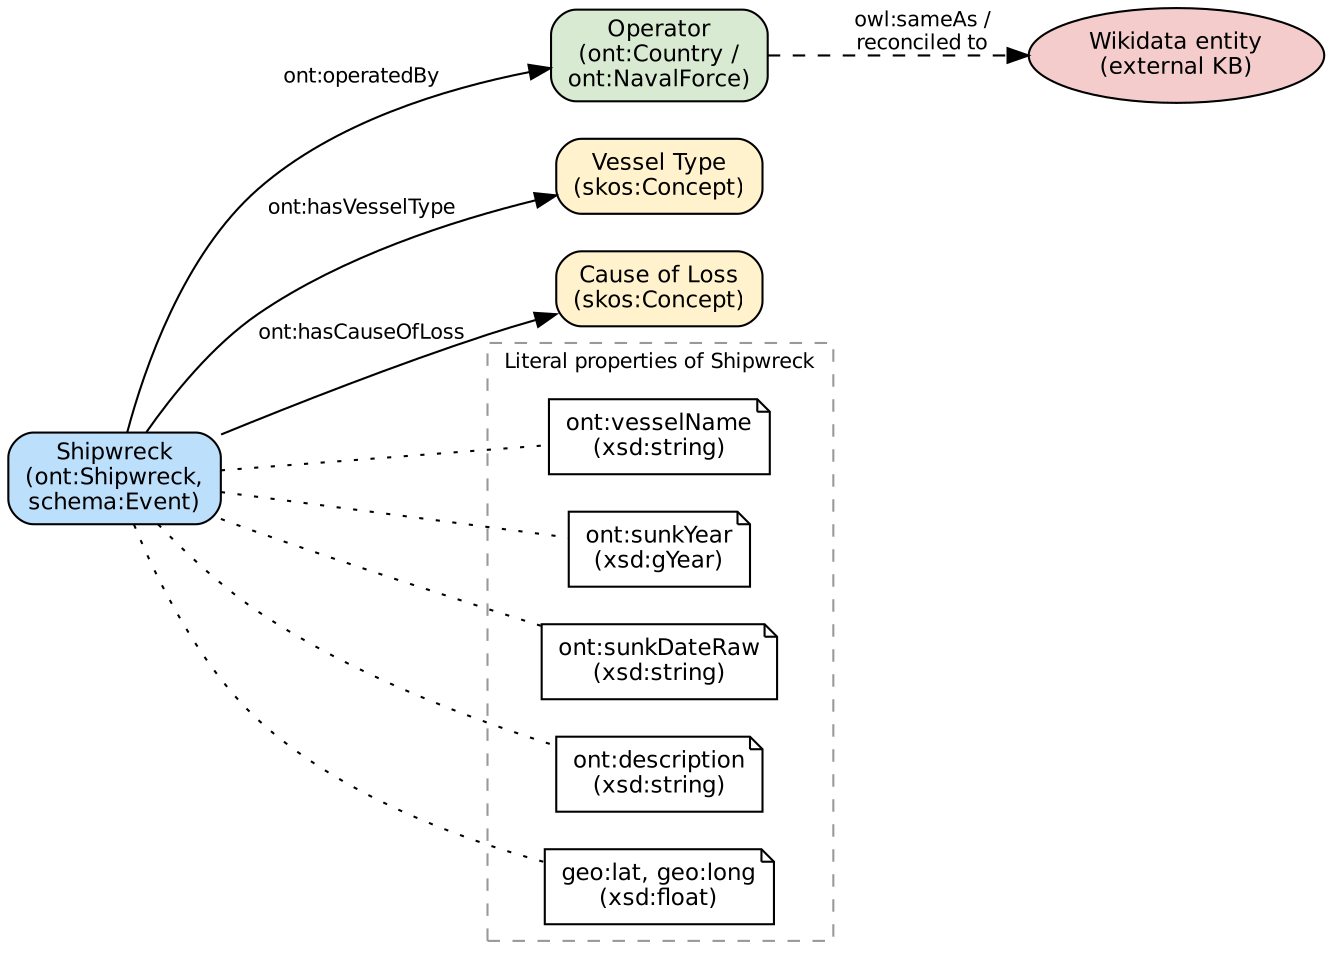
\includegraphics[width=0.95\textwidth]{semantic_model.png}
    \caption{Semantic data model for the FAIRified Shipwrecks dataset (Group 26). Dashed items are literal/datatype properties; the dashed arrow to Wikidata represents reconciliation performed during triplification.}
    \label{fig:semmodel}
\end{figure}

Our ontology IRI is \url{https://w3id.org/FAIR-course-UT/2026/group26/ont}, with concepts such as \url{https://w3id.org/FAIR-course-UT/2026/group26/ont#Shipwreck}.

\subsection{Data triplification}

Rather than performing the RDF transformation manually through OpenRefine's RDF extension (the GUI route), we implemented an equivalent, reproducible \textbf{RDF-generation script} (Python, using the \texttt{rdflib} library) -- an approach explicitly allowed by the project instructions as an alternative to OpenRefine. The script:

\begin{enumerate}
    \item Reads the cleaned, coordinate-complete subset (943 rows) produced during data preparation.
    \item Mints one subject URI per shipwreck under our Base URI, \url{https://w3id.org/FAIR-course-UT/2026/group26/data#}, e.g. \url{https://w3id.org/FAIR-course-UT/2026/group26/data#shipwreck-1012-hms-amphion}.
    \item Asserts \texttt{rdf:type ont:Shipwreck} and \texttt{schema:Event}, plus the literal properties (name, year, raw date, description, coordinates).
    \item For the \texttt{Flag} (Operator) value, checks a manually curated reconciliation table of the most frequent values ($\geq$20 occurrences) against Wikidata; a match links \texttt{ont:operatedBy} directly to the Wikidata entity (e.g. \texttt{wd:Q172771} for the Royal Navy). Unmatched values are still represented, as a locally-typed \texttt{ont:Country} or \texttt{ont:NavalForce} resource carrying the same label, so no information is silently dropped.
    \item Links each shipwreck to its \texttt{ont:VesselType} and \texttt{ont:CauseOfLoss} controlled-vocabulary concept, derived earlier during data preparation via keyword matching on the free-text \texttt{Notes} field.
\end{enumerate}

Running the script over the 943-row subset produced \textbf{10,621 RDF triples} in Turtle syntax. A short excerpt is shown below:

\begin{verbatim}
grp:shipwreck-1012-hms-amphion a schema1:Event,
        ont:Shipwreck ;
    rdfs:label "Sinking of HMS Amphion"@en ;
    geo1:lat "52.116667"^^xsd:float ;
    geo1:long "2.366667"^^xsd:float ;
    ont:description "An Active-class scout cruiser sunk by a mine
        laid by SS K\"onigin Luise."^^xsd:string ;
    ont:hasCauseOfLoss ont:CauseOfLoss_mined ;
    ont:hasVesselType ont:VesselType_cruiser ;
    ont:operatedBy wd:Q172771 ;
    ont:sunkDateRaw "6-Aug-14"^^xsd:string ;
    ont:vesselName "HMS Amphion"^^xsd:string .
\end{verbatim}
